\documentclass{article}[a4]
\usepackage[utf8]{inputenc}
\usepackage{authblk}
\usepackage{tabularx}
\usepackage{url}
\usepackage{verbatimbox}
\usepackage{graphicx}
\graphicspath{{images/}}

\providecommand{\keywords}[1]
{
  \small	
  \textbf{\textit{Keywords---}} #1
}

\title{Proposal for Automatic Extraction Framework of Superconductors related Information from Scientific literature}

\author[1]{Luca Foppiano\thanks{FOPPIANO.Luca@nims.go.jp}}
\author[1]{Thaer M. Dieb\thanks{MOUSTAFADIEB.Thaer@nims.go.jp}}
\author[1]{Akira Suzuki\thanks{SUZUKI.Akira3@nims.go.jp}}
\author[1]{Masashi Ishii\thanks{ISHII.Masashi@nims.go.jp}}
\affil[1]{Research and Services Division of Materials Data and Integrated System (MaDIS), National Institute for Materials Science (NIMS), 1-2-1 Sengen, Tsukuba, Ibaraki 305-0047, Japan}

% \date{April 2019}

\begin{document}

\maketitle

\begin{abstract}
The automatic collection of materials information from research papers using Natural Language Processing (NLP) is highly required for rapid materials development using big data, namely materials informatics (MI). The difficulty of this automatic collection is mainly caused by the variety of expressions in the papers, a robust system with tolerance to such variety is required to be developed. In this paper, we report an ongoing interdisciplinary work to construct a system for automatic collection of superconductor-related information from scientific literature using text mining techniques. We focused on the identification of superconducting material names and their critical temperature (Tc) key property. We discuss the construction of a prototype for extraction and linking using machine learning (ML) techniques for the physical information collection. From the evaluation using 500 sample documents, we define a baseline and a direction for future improvements.
\end{abstract}
\keywords{material informatics, superconductors, machine learning, nlp, tdm}

\section{Introduction}
% What is the problem we are trying to solve? What are the motivation behind this project?
Automatic information extraction from research papers using Natural Language Processing (NLP) is a highly required approach in many domains. In material research, the use of big data obtained experimentally, known as Material Informatics (MI), may give insight leading to new breakthroughs in materials discovery. 
The increasing availability of scientific papers and the expertise costs to manually extract valuable data justify the needs of Text and Data Mining (TDM) automatic approaches. Despite the general understanding of the necessity of TDM, the wide variation of writing styles and formats within in the same research topics makes this task complex.
In this paper, we propose a framework for automatic data extraction and tried an application of this system to the superconductivity scientific field.
%% How research is made and what is the point of improvements?
\textit{Superconductivity is a phenomenon of exactly zero electrical resistance and expulsion of magnetic flux fields occurring in certain materials called superconductors, under a characteristic critical temperature}~\cite{wikipedia:superconductivity}. 
Historically, high-temperature superconductors have been suddenly discovered by intuition of scientists rather than systematic consideration because of the lack of theoretical understanding \cite{klintenberg2013possible} \cite{DBLP:journals/corr/abs-1812-01995}. In this situation, data-driven exploration \cite{doi:10.1080/14686996.2018.1548885}, \cite{HAMIDIEH2018346} \cite{PhysRevMaterials.2.024802} \cite{doi:10.1021/cm503507h} would be a feasible approach to discover new superconducting materials. Since it requires huge data sets for precise prediction, high-throughput experiments, first-principle calculations, existing material databases should be used as data sources.

Currently, several material databases are available for property search. However, when looking at the superconductor sub-domain, the main one is SuperCon~\cite{SuperCon} hosted and maintained by the National Institute for Materials Science (NIMS). The SuperCon contains about 32000 inorganic and about 558 organic superconductor material definitions. Although it is constantly updated with manual data collection, it cannot catch up with the massive fresh information from the increasing number of articles each year. It is our challenge to make SuperCon richer for data-driven science.

%The research in superconductor materials is articulated toward many different objectives. Discovery of new characteristic of well known materials, under new environment condition, like applied pressure or magnetic field. Combination of known superconductors with non-superconductors may lead to new materials with better characteristics, usually a higher critical temperature. 

% Add that introduction about the available databases, in particular NIMS, which has the problem that is not updated due to high costs of manual work
%Currently there are several general material databases available, however when looking  at the superconductor sub-domain the main one is SuperCon\cite{SuperCon}. Hosted and maintained by the National Institute for Materials Science (NIMS) containing about 32k inorganic and about 558 organic superconductor material definitions. Although the update continues manually, the latest information can not keep up with the increase in the enormous number of articles each year. 

% Why do we need such information? Why these information are important?
%The availability of material information with detailed and precise granularity is a must-have for superconductors scientists. This data summarises decades of research and discoveries and can be potentially exploited in many areas. Machine learning or neural models can train generative models specialised in automatically predict critical temperature \cite{DBLP:journals/corr/abs-1812-01995} on new (pure or intercalated) materials. Large scale repositories with enhanced search specialised in semantic superconductor disambiguation, document recommendation, and so on. 

In this paper, we describe the ongoing attempt to design a TDM system using NLP techniques. In particular, we focus on extracting superconducting materials names and their linking to the corresponding critical temperature (Tc) values. Our system is built on an open source library for text mining for scholarly documents: Grobid~\cite{GROBID}. We evaluate the performance of the system using precision, recall and F1-score. These quantitative values provide a baseline for measuring our progress in solving the task. Similar attempts of mining scientific literature in materials domain had been conducted in \cite{nanocrystal_extraction} \cite{court2018auto}. 

This paper is organised as follows, Section~\ref{sec:architecture} describes the details of a working prototype specialised in which development of annotated corpus for material name recognition is included. Section~\ref{sec:experiments-results} presents the evaluation methods and results. Section~\ref{sec:conclusion} concludes this paper with summary and scopes.

\section{System architecture}
\label{sec:architecture}
The scientific information in articles is often presented in tables and figures for easy understanding. However, in order to achieve higher order data structuring, it is necessary to link extracted entities. For example, the different expressions of superconductor’s name should be appropriately linked to corresponding property values depending on various material and measurement parameters, where the material parameter is the dopant density, stoichiometry, etc. and measurement parameter is the applied magnetic field, pressure, and so on. Obviously, these relational entities are not fully included in the tables and figures. Therefore, we insist on extracting information existing in the main body text and in captions of tables and figures. In superconductor sub-domain, since a dataset of superconductor material and its corresponding Tc is crucial, we constructed a system for linking the material and Tc (material-Tc). Other properties, such as critical magnetic field (Hc) will be targeted in the upcoming work.

We built our implementation based on an open source library called Grobid \cite{GROBID}. Grobid is a sequence labelling and document segmentation library based on machine learning (ML), Conditional Random Field (CRF) \cite{lafferty2001conditional}. It provides full support for extraction of data from PDF and built-in workflow for pre-annotating training data, machine learning models training and evaluation. The PDF support in Grobid was important because allowed us to focus on the processing of a single format instead of dealing with several XML flavours depending on external publishers. Among various available open source tools, the choice of Grobid is well justified by the fact that it is still actively developed and it is available as ready product employed in several large-scale research repositories, such as Mendeley \cite{mendeley-extraction}. In a recent benchmark study, Grobid performed best in citation extraction task  \cite{DBLP:journals/corr/abs-1802-01168}. Lastly, Grobid has
been successfully extended to support several domain specific problems, for example, astronomical entities recognition \cite{grobid-astro}, dictionaries segmentation \cite{khemakhem2017automatic}, software mention \cite{software-mentions} and measurements extraction and normalisation \cite{grobid-quantities}. Such open source measurement extractor, Grobid-quantities was fitting in our use case for Tc recognition.

\begin{figure}[]
    \centering
    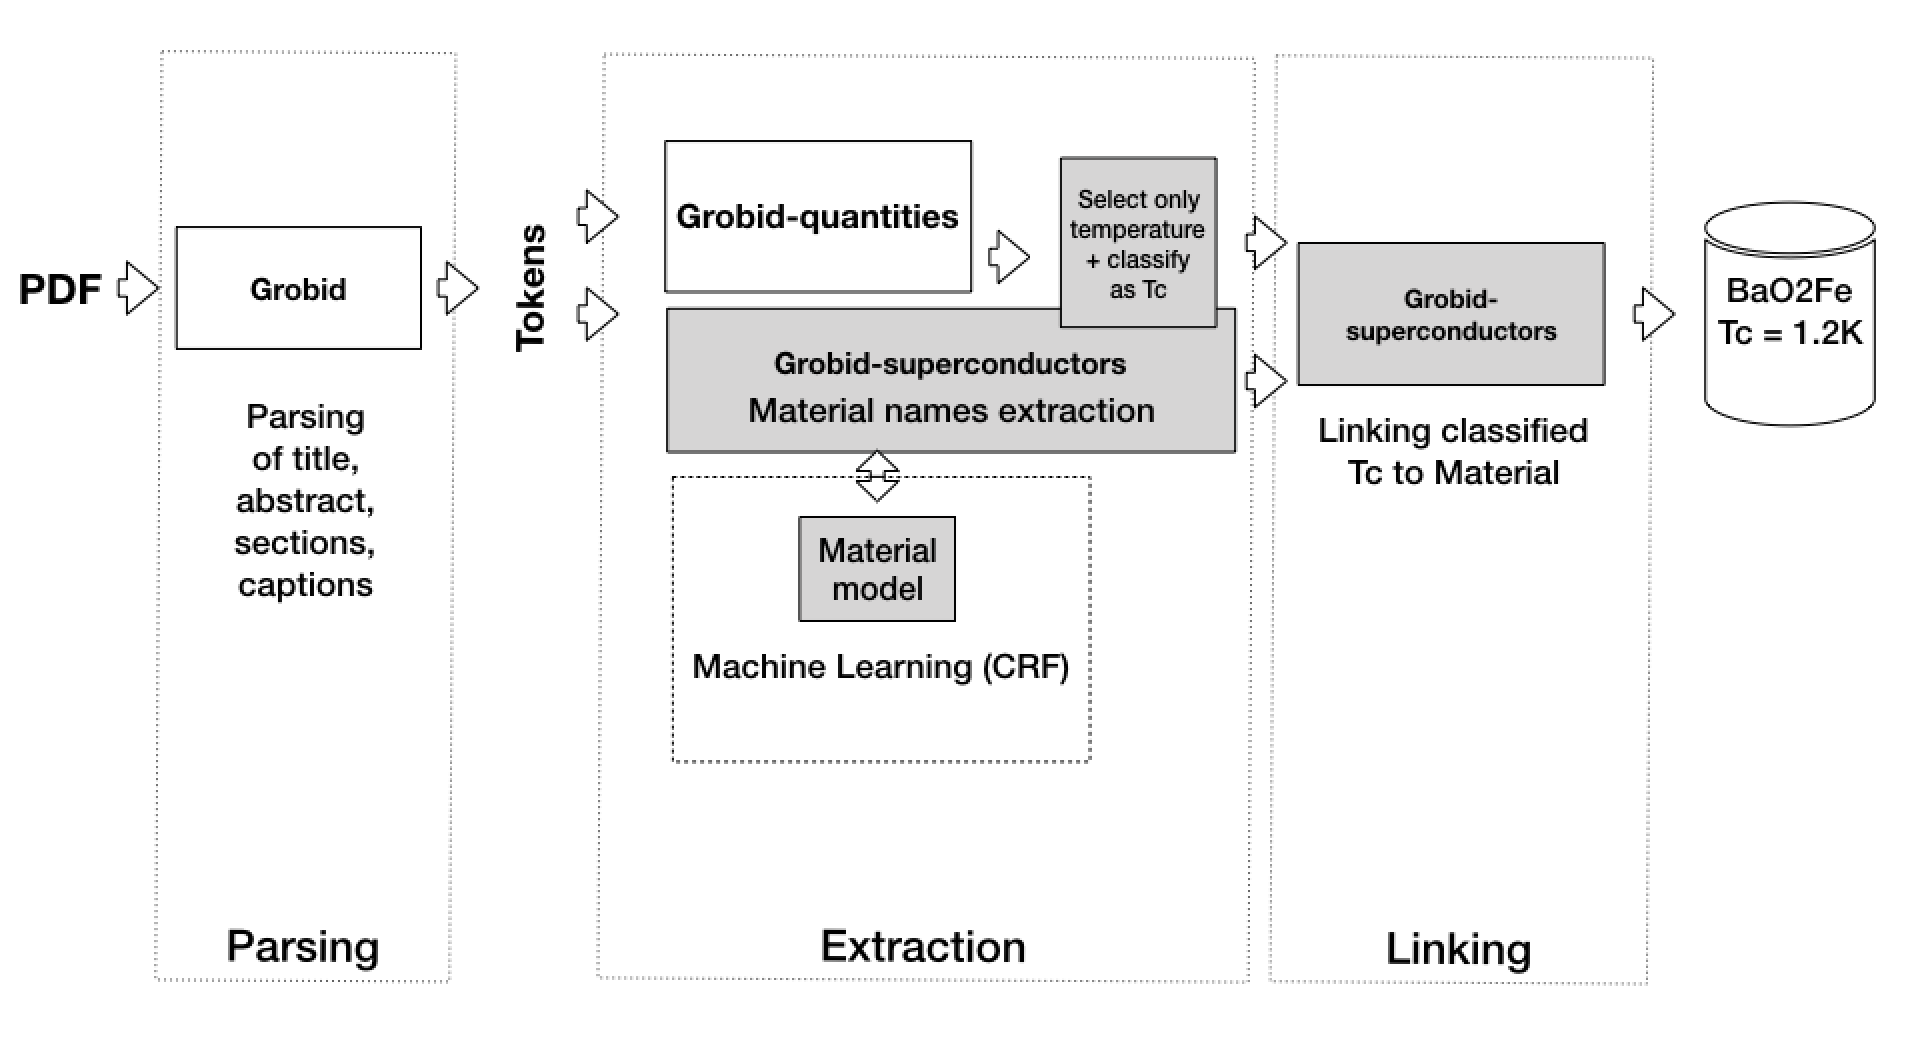
\includegraphics[width=4in]{schema}
    \caption[Schema of the system] {Schema of the system}
    \label{fig:system-schema}
\end{figure}

Our developed system illustrated in Figure \ref{fig:system-schema}, it consists mainly of two phases: (a) “Extraction phase” and (b) “Linking phase”. We extract relevant entities, i.e., superconducting materials and Tc in (a), and link these extracted entities in (b). After parsing title, abstract, sections, and captions and following tokenisation, the (a) Extraction phase combines the entities resulting from a newly trained model for superconductor material recognition and a conventional module, Grobid-quantities for measurement extraction. The superconducting material recognition model was trained with five full documents manually annotated (42 entity in total). We also used domain-specific chemical recogniser, called ChemSpot \cite{10.1093/bioinformatics/bts183} which extracts chemical entities from text and classify them into types: SYSTEMATIC, IDENTIFIER, FORMULA, TRIVIAL, ABBREVIATION, FAMILY, MULTIPLE and UNKNOWN.

In the following (b) Linking phase, three tasks are sequentially performed. Since Grobid-quantities supports extraction of a wide range of measurements (temperatures, lengths, pressures, etc.), we selected only temperatures (task 1, Selection). Then we classified each of them into “Tc” and the others (task 2, Classification). Finally, we linked “Tc” with the positionally closest material term (task 3, Linking). The (2) classification was realised by word matching to an original dictionary which summarises commonly used as Tc-related words in superconducting literature (e.g. “Tc”, “critical temperature”). We looked for the Tc-related words in the surroundings (within five words according to empirical probability) of a numerical temperature value and made a pair of Tc and value (Tc-value). At last, we (3) linked the closest material term to Tc- value, resulting in the required entity linking of material-Tc-value.

In Figure~\ref{fig:example-working} and Figure~\ref{fig:example-not-working} we show two examples each of correct and incorrect linking respectively. Figure~\ref{fig:example-working} indicates the automatic links of material (Figure~\ref{fig:example-working}a) BaTi\textsubscript{2}Bi\textsubscript{2}O with Tc of 4.6K and (Figure~\ref{fig:example-working}b) BaTi\textsubscript{2}Sb\textsubscript{2}O with 1.2K. Figure 3, however, shows (Figure~\ref{fig:example-not-working}a) unlinked BaTi\textsuperscript{2}Sb\textsuperscript{2}O to the Tc-value and (Figure~\ref{fig:example-not-working}b) the incomplete linking of KO\textsuperscript{S2}O\textsubscript{6} to the Tc-value. In the former case, the misclassification of 1.2K in task 2 results in unlinked BaTi\textsuperscript{2}Sb\textsuperscript{2}O. In the latter case, misrecognition of a decimal point as a period provided an incomplete Tc value of 60K. The statistical investigation of the (b) Linking phase is discussed in the later part of Section 3.

%We limited the search span at \textit{sentence level} and \textit{paragraph level} by constraining the search at the same sentence or at the same paragraph respectively (Table \ref{table:result-linking}).

\begin{figure}[h]
    \centering
    (a) \\
    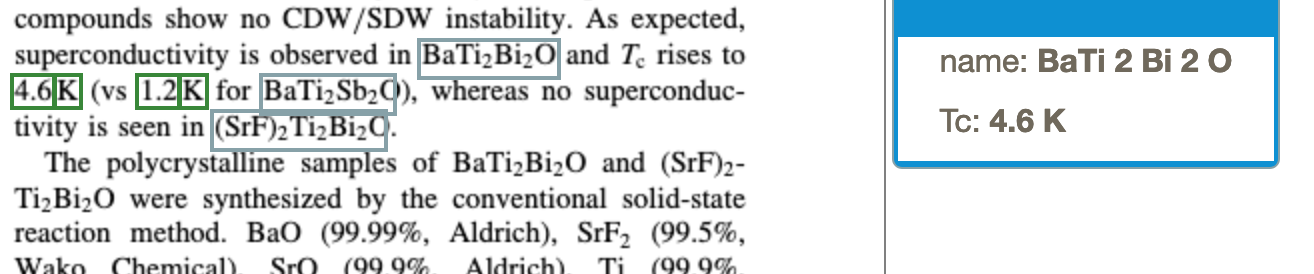
\includegraphics[width=4in]{example1} \\
    (b) \\
    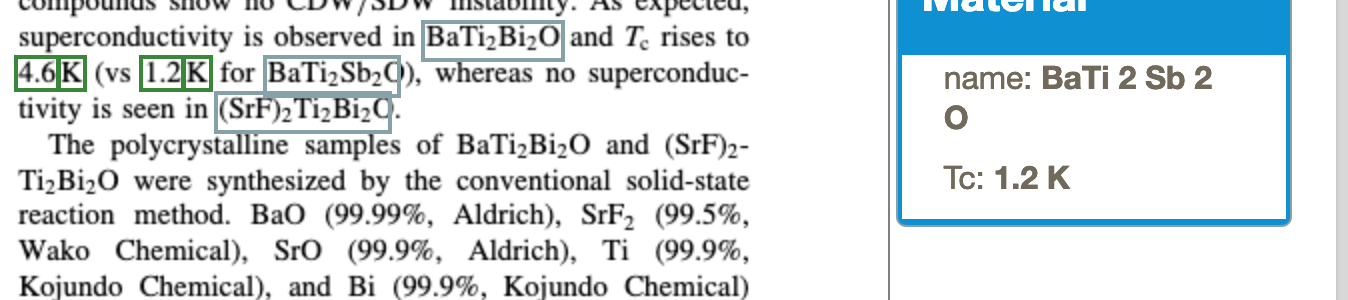
\includegraphics[width=4in]{example2}
    \caption{Example of a correct linking between material and Tc. The popup windows indicate the links of material (a) BaTi\textsubscript{2}Bi\textsubscript{2}O with Tc of 4.6K and (b) BaTi\textsubscript{2}Sb\textsubscript{2}O with 1.2K.}
    \label{fig:example-working}
\end{figure}

\begin{figure}[h]
    \centering
    (a) \\
    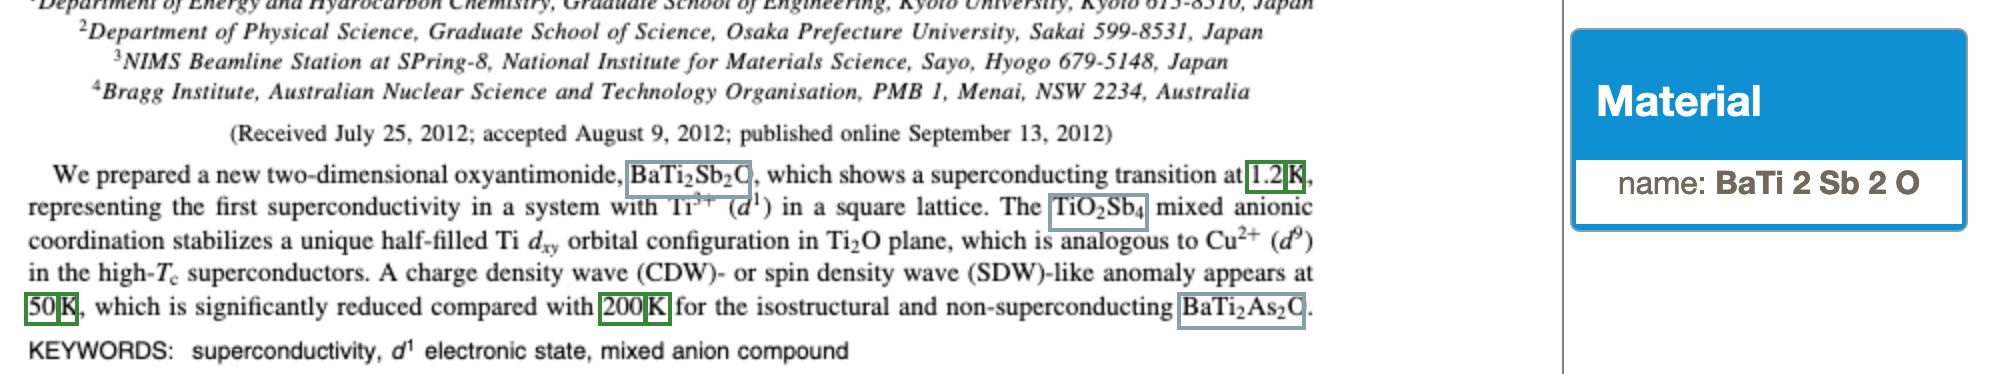
\includegraphics[width=4in]{example-bad1}  \\
    (b) \\
    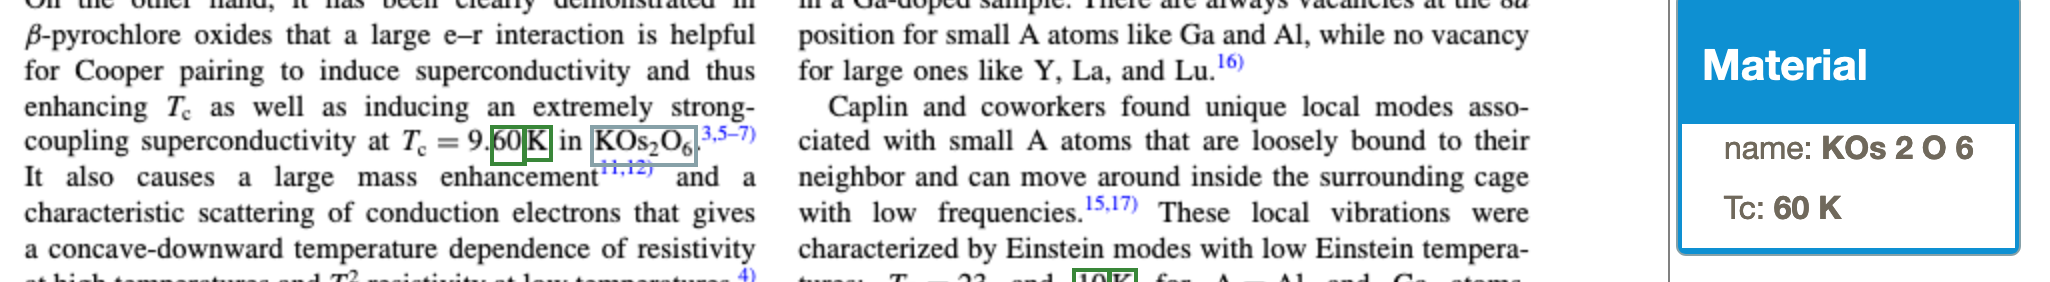
\includegraphics[width=4in]{example-bad2}
    \caption{Example of an incorrect linking between material and Tc. Although the materials (a) BaTi\textsuperscript{2}Sb\textsuperscript{2}O and (b) KO\textsuperscript{S2}O\textsubscript{6} are correctly identified, Tc of BaTi\textsuperscript{2}Sb\textsuperscript{2}O cannot be extracted and that of KO\textsuperscript{S2}O\textsubscript{6} is extracted incorrectly (correct Tc was 9.60 K while the extracted value was 60 K).}
    \label{fig:example-not-working}
\end{figure}

\section{Experiments and results}
\label{sec:experiments-results}
The superconductor CRF model in the (a) Extraction phase was investigated using a corpus of five papers (four for training and one for testing) having a total of 42 entities classified with a superconducting material label \textless supercon\textgreater.

\begin{figure}[h!]
    \centering
    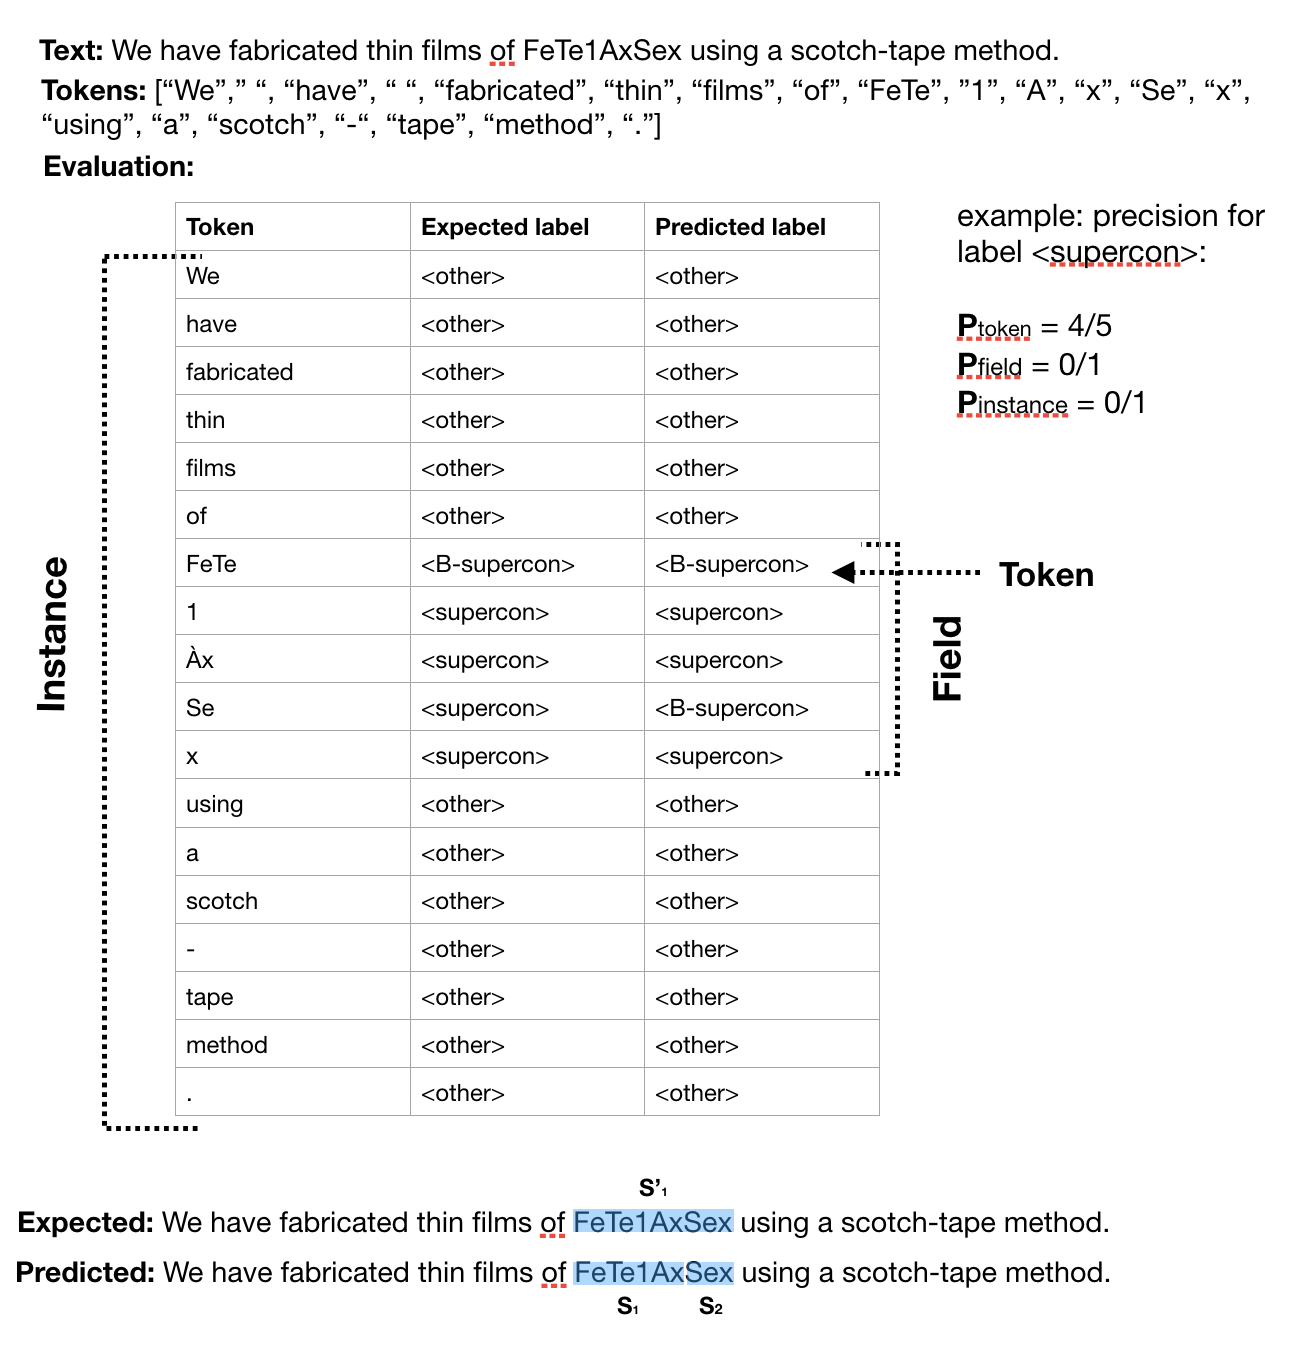
\includegraphics[width=4in]{example-output}
    \caption{Given a sentence (or paragraphs) the tokenisation transforms it in an array of character sequences. These are then labelled by the ML CRF model. This figure illustrates the three different levels of granularity on which measurements are calculated.}
    \label{fig:levels-measurement}
\end{figure}

We estimated precision, recall and F1-score for the model using the evaluation framework built-in in Grobid. These measure indices are calculated at three different levels: tokens-level, field-level and instance-level. Figure \ref{fig:levels-measurement} the concept through an example of prediction. In this table, expected (second column) and predicted (third column) labels are tagged on to each token. The token-level evaluates the predictability for each token P\textsubscript{token}, in this example equals to 4/5. The field-level evaluates the continuity of a field with the same label. Although “FeTe\textsubscript{1}A\textsubscript{x}Se\textsubscript{x}” should be recognised as a field, the predicted label indicated separation into two fields of “FeTe\textsubscript{1}A\textsubscript{x}” and “Se\textsubscript{x}”. Therefore, the predictability in field-level, P\textsubscript{field} is 0/1. Finally, instance-level indicates predictability of the continuity of all the fields within the same instance, where the instance is defined by a paragraph in this case. If “FeTe\textsubscript{1}A\textsubscript{x}Se\textsubscript{x}” is only one field in the paragraph, the predictability in instance-level, P\textsubscript{instance} is 0/1. The predictability of P\textsubscript{token}, P\textsubscript{field}, and P\textsubscript{instance} are statistically extendable to more strict indices of precision, recall, and F1-score.

\begin{table}[h!]
    \centering
    \caption{Grobid evaluation framework results (precision, recall and F1-score) for the (a) material extraction}   
    \begin{tabular}{ | m{7em} | m{5em} | m{5em} | m{5em} | m{5em} | }
        \hline
        \multicolumn{5}{|c|}{\textbf{Token-level results}} \\
        \hline
        Label & Accuracy & Precision & Recall & F1 \\
        \hline
        \textless supercon\textgreater & 98.61 & 84.42 & 85.28 & 84.85 \\
        \hline
        \multicolumn{5}{|c|}{\textbf{Field-level results}} \\
        \hline
        Label & Accuracy & Precision & Recall & F1 \\
        \hline
        \textless supercon\textgreater & 72.94 & 66.67 & 56.25 & 61.02 \\
        \hline
        \multicolumn{5}{|c|}{Instance-level results} \\
        \hline
        \multicolumn{5}{|c|}{
            \begin{tabular}{ c | c | c }
                Total expected instances & Correct instances & Instance-level recall \\
                \hline 
                22 & 15 & 68.18 \\
            \end{tabular}
        } \\
        \hline
    \end{tabular}
    \label{table:result-extraction-grobid}
\end{table}

As shown in Table \ref{table:result-extraction-grobid}, recall at token-level, field-level, and instance-level were 85.28, 56.25, and 68.18\%, respectively. The minimum recall at the field-level indicates insufficient training for recognition of superconducting compounds, rather than superconducting elements. The higher score at instance-level suggests that some specific superconducting compounds which are intensively appeared in a paragraph have never been trained at this stage. Moreover, the fact that the precision (66.67\%) is better than the recall (56.25\%) in the field-level indicates false positive (FP) is smaller than false negative (FN). Consequently, the true superconducting compounds are relatively difficult to recognise for our trained model (c.f., Figure~\ref{fig:levels-measurement}). We have already found that missing annotation in the training papers, and so a quality improvement of training data is necessary to establish a practical extraction system.

Finally, we tested the proposed system on a larger corpus of papers. We processed 500 superconductor-related PDF papers from three publishers: American Institute of Physics (AIP), American Physical Society (APS) and Institute of Physics (IOP) and we manually evaluated the extracted critical temperatures and their link with the related material. As discussed in Figure~\ref{fig:levels-measurement} the material recognition in (a) the Extraction phase mistook in boundaries detection. The other examples of mistake are \textit{missing notation}: predicted LaFe\textsubscript{x}O for expected LaFe\textsubscript{x}O\textsubscript{1-x}, and \textit{irregular separation}: predicted single superconductor for expected two different materials separated by coordinating conjunctions like “and” or “comma”.
Despite several imperfect extractions, we obtained unique material entities of 1644 from the 500 papers as summarised in Table \ref{table:result-extraction}. For Tc extraction, although the temperature could refer to unrelated experimental conditions or thermal treatment for sample preparation, the number of extracted Tc was 1173.

\begin{table}[h!]
    \centering
    \caption{Material and Tc extraction results from a corpus of 500 papers.}    
    \begin{tabular}{ | m{4em} | m{4em} | m{6em} | m{5em} | } 
    \hline
        Material entities & Unique material entities & Temperature entities & Tc entities \\
    \hline
        5400 & 1644 & 7554 & 1173 \\ 
    \hline
    \end{tabular}
    \label{table:result-extraction}
\end{table}

Table \ref{table:result-linking} shows evaluations at \textit{sentence-level} and \textit{paragraph-level} for the (b) Linking phase. As shown in this table, 77 (sentence-level) and 109 (paragraph-level) correct links are obtained for the extracted Tc of 1173. From these values, in the case of sentence-level boundary, precision and recall were estimated to be 68.7\% and 6.5\%, respectively. The paragraph-level resulted in lower precision and higher recall, 57\% and 10.7\% respectively. Increasing the search span from sentence to paragraph, F1-score increased from 11.87\% to 18.01\%. The decrease in precision was compensated by the increase in recall.
The generally low recall is partly caused by wrong parsing prior to (a) Extraction phase. The conversion from PDF to text unavoidably produces irregular tokens originated from wrong UTF-8 characters, stream-ordering issues, and missing fonts. Considering that we used empirical rules for linking as described in Section~\ref{sec:architecture}, the irregular tokens increase FN, resulting in the low recall. The effects of irregular tokens can be reduced by using volumes of training data with a high-quality corpus.

\begin{table}[h!]
    \centering
    \caption{Result of linking materials and Tc.}   
    \begin{tabular}{ | m{7em} | m{4em}| m{4em}| m{4em}| m{4em} | m{4em} | } 
    \hline
        Boundaries & Links & Correct links & precision & recall & F1-score \\
    \hline
            sentence-level  & 112 & 77 & 68.7\% & 6.5\% & 11.87 \% \\
    \hline
            paragraph-level & 191 & 109 & 57\% & 10.7\% & 18.01 \% \\
    \hline
    \end{tabular}
    \label{table:result-linking}
\end{table}

\section{Conclusion}
\label{sec:conclusion}
In this paper, we proposed an automatic extraction of superconductor related information from scientific publications. The proposed system consists of two phases: a machine learning sequence labelling process for entity extraction (Extraction phase) and a simple rule-based for linking (Linking phase).
Although we found feasible performance for the (a) Extraction phase using a sequence labelling approach, bulk corpus is necessary to reach practical performances. For the (b) Linking phase, the rule-based approach was limited by irregular tokens introduced in a conversion process from PDF to text, so that probability model and ML are required. In the next step, we plan to introduce deep neural networks like Bi-LSTM+CRF approach and embedding in the Extraction phase.

\pagebreak

\bibliography{references}
\bibliographystyle{unsrt}

\end{document}
